% Created 2017-03-30 Thu 11:09
\documentclass[10pt,t,a4paper]{beamer}
\usepackage[utf8]{inputenc}
\usepackage[T1]{fontenc}
\usepackage{fixltx2e}
\usepackage{graphicx}
\usepackage{longtable}
\usepackage{float}
\usepackage{wrapfig}
\usepackage{rotating}
\usepackage[normalem]{ulem}
\usepackage{amsmath}
\usepackage{textcomp}
\usepackage{marvosym}
\usepackage{wasysym}
\usepackage{amssymb}
\usepackage{hyperref}
\tolerance=1000
\usetheme{BTH_msv}
\author{Mikael Svahnberg\thanks{Mikael.Svahnberg@bth.se}}
\date{2017-03-30}
\title{Software Testing}
\hypersetup{
  pdfkeywords={},
  pdfsubject={},
  pdfcreator={Emacs 25.1.1 (Org mode 8.2.10)}}
\begin{document}

\maketitle

\begin{frame}[label=sec-1]{Testing Goals}
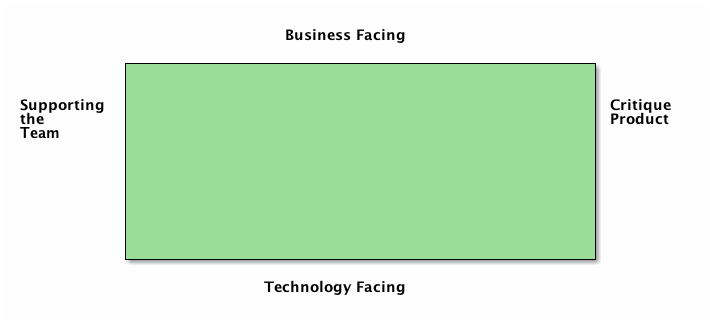
\includegraphics[width=.9\linewidth]{./FTestQuadrants1.png}

{\tiny
(L. Crispin and J. Gregory, ``Agile Testing -- A Practical Guide for Testers and Agile Teams'', Pearson Education, 2009.)
}

\alert{Discuss:} What types of testing can you expect to see in each corner of this square?
\end{frame}

\begin{frame}[shrink=15,label=sec-2]{Lower Left Quadrant: Technology Facing / Supporting the Team}
\begin{itemize}
\item Testability of
\begin{itemize}
\item API's,  Ports, Adapters
\end{itemize}
\item Test database access, updates
\item Business Logic and Presentation separated
\item Isolated tests
\begin{itemize}
\item to isolate problems
\end{itemize}
\item Internal Quality
\item Infrastructure
\end{itemize}

Safety Net!
\begin{itemize}
\item build confidence
\item go faster, do more
\item support refactoring
\end{itemize}
\begin{block}{Examples of Techniques}
\begin{itemize}
\item Unit Tests
\item Component Tests
\end{itemize}
\end{block}
\end{frame}
\begin{frame}[label=sec-3]{What, Who, When?}
\begin{itemize}
\item Unit Tests
\begin{itemize}
\item Developer Intent and program design
\item Does the code-in-the-small do what it is expected to do
\end{itemize}
\item Component Tests
\begin{itemize}
\item Architect's intents -- system design
\item Do components work together as expected
\end{itemize}
\item The \alert{Programmer} writes the test and test them
\item Run tests in Continuous Integration tool
\end{itemize}
\end{frame}
\begin{frame}[label=sec-4]{Toolkit}
\begin{itemize}
\item Source Code Management
\begin{itemize}
\item Version Control
\item Who changed what?
\item Be able to restore to older version
\end{itemize}
\item IDE
\begin{itemize}
\item Compile, Debug, Build GUI, Unit Test, Refactor
\end{itemize}
\item Unit Tests
\begin{itemize}
\item e.g. xUnit
\end{itemize}
\item CI tools
\begin{itemize}
\item e.g. Jenkins, Travis.ci, Drone.io, $\ldots$
\end{itemize}
\end{itemize}
\end{frame}
\begin{frame}[shrink=15,label=sec-5]{Upper Left Quadrant: Business Facing / Support the Team}

\begin{itemize}
\item Drive Development with business-facing tests
\item Ask the right questions
\item Help customers clarify
\item Captuer examples, express as executable tests
\item External Quaity
\item Know when we're done.
\end{itemize}
\begin{block}{Examples of Techniques}
\begin{itemize}
\item Functional Tests
\item Examples
\item Story Tests
\item Prototypes
\item Simulations
\end{itemize}
\end{block}
\end{frame}
\begin{frame}[label=sec-6]{What, Who, When?}
\begin{itemize}
\item Testers, Developers
\item Collaboration with customers
\item Team responsibilty
\item Start of Iteration
\begin{itemize}
\item Business facing tests drive development
\end{itemize}
\item Throughout Iteration
\begin{itemize}
\item No story done until tested
\end{itemize}
\end{itemize}
\end{frame}
\begin{frame}[label=sec-7]{Toolkit}
\begin{itemize}
\item Checklists
\item Mind Maps
\begin{itemize}
\item Brainstorming
\item Words, ideas, tasks
\end{itemize}
\item Mockups / Paper Prototypes
\begin{itemize}
\item User-centered design
\end{itemize}
\item Flow Diagrams
\item Whiteboards
\item Behaviour-Driven-Development
\begin{itemize}
\item Cucumber, easyB, nbehave, rspec
\end{itemize}
\item GUI Test tools/libraries/frameworks
\begin{itemize}
\item e.g. Selenium, Cucumber, Canoo WebTest, Robot Framework $\ldots$
\end{itemize}
\end{itemize}
\end{frame}
\begin{frame}[label=sec-8]{Upper Right Quadrant: Business Facing / Critique Product}
\begin{itemize}
\item Recreate actual user experiences
\item Realistic use
\item Learn as you test
\item Context
\begin{itemize}
\item What works for your situation
\end{itemize}
\item Constructive
\end{itemize}
\begin{block}{Examples of Techniques}
\begin{itemize}
\item Customer Demos
\item Exploratory Testing
\item Scenarios
\item Usability Testing
\item User Acceptance Testing
\item Alpha/Beta Testing
\end{itemize}

\alert{Discuss} How does this relate to UML and RUP?
\alert{Discuss} Are these tests automated or manual?
\end{block}
\end{frame}
\begin{frame}[label=sec-9]{Also behind the GUI}
\begin{itemize}
\item Test API
\begin{itemize}
\item Input/Output
\item Sequence of API calls
\item Checking log files
\item States and Transitions
\end{itemize}
\end{itemize}
\end{frame}
\begin{frame}[label=sec-10]{What Who, When?}
\begin{itemize}
\item Require good skills, experience, intuition, critical thinking
\item Invole the customers
\item As early as possible
\end{itemize}
\end{frame}
\begin{frame}[label=sec-11]{Toolkit}
\begin{itemize}
\item Time
\item Experience
\item Some of upper left quadrant tools may apply
\begin{itemize}
\item e.g. Selenium, Cucumber, Canoo WebTest, Robot Framework $\ldots$
\end{itemize}
\end{itemize}
\end{frame}
\begin{frame}[label=sec-12]{Lower Right Quadrant: Technology Facing / Critique Product}
Quality Attributes, e.g.:
\begin{itemize}
\item Performance
\item Stability
\item Reliability
\item Scalability
\item Maintainability
\item $\ldots$
\end{itemize}

Also
\begin{itemize}
\item Memory Management
\item Data Migration
\item Recovery
\end{itemize}

Test Environment
\begin{itemize}
\item Independent, production-like environment
\end{itemize}
\end{frame}
\begin{frame}[label=sec-13]{What, Who, When?}
\begin{itemize}
\item Depends on priorities
\item May be needed already from the get-go
\item At least get an early baseline
\end{itemize}
\end{frame}
\begin{frame}[label=sec-14]{Toolkit}
\begin{itemize}
\item Data Migration, Recovery:
\begin{itemize}
\item Native Database Tools
\item Shell Scripts
\end{itemize}
\item Monitoring tools
\begin{itemize}
\item jConsole : Application bottlenecks, memory leaks
\item jProfiler: Database usage
\end{itemize}
\item Load Tests
\begin{itemize}
\item Loadrunner, SilkPerformer
\end{itemize}
\item Other tools
\begin{itemize}
\item jMeter, jUnitPerf, $\ldots$
\end{itemize}
\end{itemize}
\end{frame}
\begin{frame}[label=sec-15]{Test Quadrants, Summary}
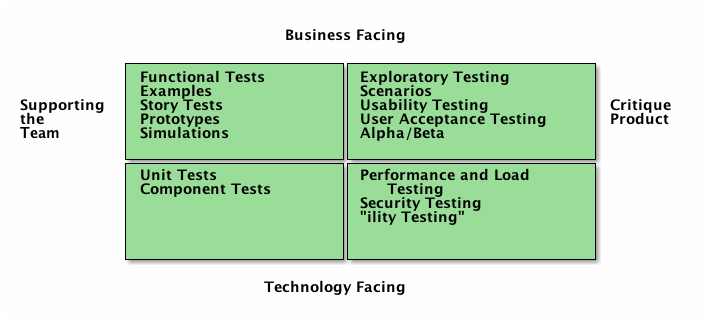
\includegraphics[width=.9\linewidth]{./FTestQuadrants0.png}
\end{frame}

\begin{frame}[label=sec-16]{Plan your Test Strategy}
\begin{itemize}
\item Scope
\item Priorities, Risks
\item Tools
\item Customers
\item What to Document
\item Consider all four quadrants
\item Use lessons learned to improve
\end{itemize}
\end{frame}
\begin{frame}[label=sec-17]{TDD: Test Driven Development}
\emph{nano-cycle} (second by second)
Three laws of TDD:
\begin{enumerate}
\item You must write a failing test before you write any production code.
\item You must not write more of a test than is sufficient to fail, or fail to compile.
\item You must not write more production code than is sufficient to make the currently failing test pass.
\end{enumerate}

\emph{micro-cycle} (minute by minute)
Red-Green-Refactor cycle

\begin{enumerate}
\item Create a unit tests that fails
\item Write production code that makes that test pass.
\item Clean up the mess you just made.
\end{enumerate}
\end{frame}
\begin{frame}[label=sec-18]{TDD: Test Driven Development}
\emph{milli-cycle} (10 minute intervals)
\begin{itemize}
\item More specific test cases $\rightarrow$ more generic code
\item Code is no longer a series of special cases
\item ``Big Picture''
\item Backtrack from too specific test cases or not general enough code
\end{itemize}

\emph{primary cycle} (hour by hour)
\begin{itemize}
\item ensure architectural boundaries
\end{itemize}
\end{frame}
\begin{frame}[label=sec-19]{Discuss: Testing and RUP/UML}
\begin{itemize}
\item How does RUP/UML deal with Testing?
\item What areas do RUP/UML focus on?
\end{itemize}

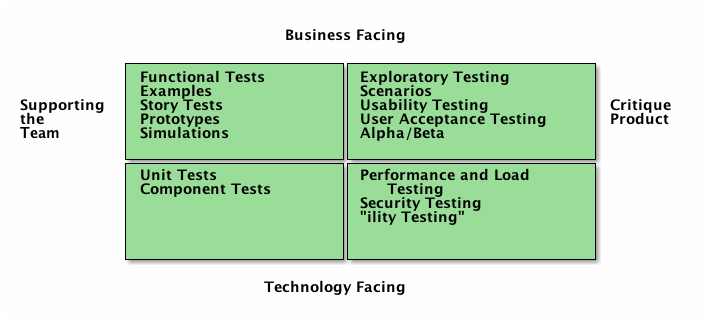
\includegraphics[width=.9\linewidth]{./FTestQuadrants0.png}
\end{frame}
% Emacs 25.1.1 (Org mode 8.2.10)
\end{document}